\documentclass[a4paper,12pt]{article}
\usepackage[utf8]{inputenc}
\usepackage[T1]{fontenc}
\usepackage[francais]{babel}
\usepackage{geometry}
\usepackage{graphicx}
\usepackage{hyperref}
\usepackage{float}
\usepackage[backend=biber]{biblatex}
\geometry{top=2cm, bottom=2cm, left=2cm, right=2cm}

\addbibresource{bibliography.bib}

\title{\textbf{Rapport Préliminaire}}
\author{Jeu de plateau: Othello - Reversi}
\date{\today}

\begin{document}

\maketitle

\tableofcontents
\newpage

\section{Présentation du projet}

Afin de nous familiariser avec la conduite de projet, nous devons cette année
développer un logiciel permettant de jouer à un jeu de plateau.\\ Comme nous
n'avons pas réellement de clients avec qui discuter de l'implémentation, nous
avons été remis un cahier des charges listant des besoins généraux qu'il nous
faudra décomposer en besoins plus spécifiques.\\

Pour ce projet, nous allons travailler en Python sur le jeu de plateau
Othello.\\ Othello, que l'on peut trouver également sous le nom Reversi -
Othello étant une marque déposée, se joue à deux joueurs sur un plateau carré
de 8x8 cases.\\ Chaque joueur possède des pions de couleur blanche ou noire.\\
Notre but ici sera d'implémenter ce jeu en langage python, et de donner une
interface graphique et des commandes additionnelles à l'utilisateur.\\

\section{Description du Projet}
\subsection{Règles du jeu}

Othello se joue sur un plateau unicolore de 64 cases: l'othellier.\\ Les deux
adversaires jouent avec 64 pions de couleur blanche d'un côté et noire de
l'autre.\\ Au tout début de la partie, quatre pions sont placés au centre du
plateau: deux pions noirs en E4 et D5, et deux pions blancs en E5 et D4.\\ Les
cases de l'othellier sont numérotées par les lettres A à H pour les colonnes,
et par les chiffres 1 à 8 pour les lignes.\\

\begin{figure}[!h]
  \centering
  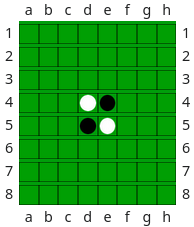
\includegraphics[width=5cm]{images/ReversiStartingPos.png}
  \caption{Position des pions au départ}
\end{figure}

Les joueurs jouent chacun leur tour, en commençant par le joueur aux pions
noirs.\\ Ils doivent capturer les pions de leur adversaire à chaque tour.\\ Si
le joueur ne peut pas capturer de pion, il passe son tour.\\ Un pion placé doit
être adjacent à au moins un autre pion (de même couleur ou de couleur adverse)
dans sa ligne, colonne ou diagonale.\\

Une capture se produit lorsque le joueur dont c'est le tour place un pion qui
enferme un alignement (en colonne, ligne, ou diagonale) de pions adverses
(l'autre extrémité étant fermée au cours d'un tour précédent).\\ En plaçant son
pion, le joueur retourne les pions qu'il capture, les changeant en sa
couleur.\\ Si le pion posé permet de capturer plusieurs alignements à la fois,
le joueur capture tous ces pions adverses.\\ Par contre, en les retournant, ces
pions ne permettent pas de capture, même s'ils encadrent des pions adverses.\\

Le jeu se termine lorsque aucun des deux joueurs ne peut poser de pion, ou que
l'othellier n'a plus aucune case vide.\\ On compte le nombre de pions de chaque
couleur sur le plateau pour déterminer le vainqueur: le joueur ayant le plus de
pions de sa couleur présents sur l'othellier.\\

\subsection{Fonctionnalités principales}
Nous avons prévu d'implémenter le jeu Reversi fonctionnel, jouable dans le
terminal de commandes, et également via une interface graphique.\\ Il sera
possible de sauvegarder et charger une partie, ainsi que l'historique des coups
joués.\\ Des modes de jeu additionnels seront présents: un mode Blitz qui
permettra d'initialiser un temps limite de jeu pour chaque joueur au début de
la partie. Ainsi qu'un mode Contest qui chargera une partie, jouera un coup et
renverra le fichier de sauvegarde du nouveau plateau.\\ Il sera possible de
jouer contre une IA, ou de faire jouer deux IA (avec le mode contest). Cette IA
sera configurable, avec un temps de réflexion, un choix des heuristiques
utilisées, et une profondeur de recherche.\\

\subsection{Structures de données utilisées}
Afin de représenter le plateau et les pions placés, nous allons utiliser des
Bitboards.\\ Nous prévoyons pour le moment d'utiliser cinq bitboards, un
représentant le board full qui sera un masque de $taille*taille$ bits, avec
$taille$ la taille du plateau (et par extension le board vide en flippant les
bits) un pour les pions noirs et un pour les pions blancs. Nous utiliserons
également deux masques pour éviter les effets de bord liés aux décalages à
droite et à gauche du plateau.\\ Ces bitboards seront stockées dans des
tuples.\\ Les tuples des coups joués et de l'état du board seront stockés dans
une pile.\\ Les parties et l'historique des coups seront sauvegardées dans des
fichiers différents, en format ASCII, et de la forme suivante:\\
\begin{figure}[H]
  \centering
  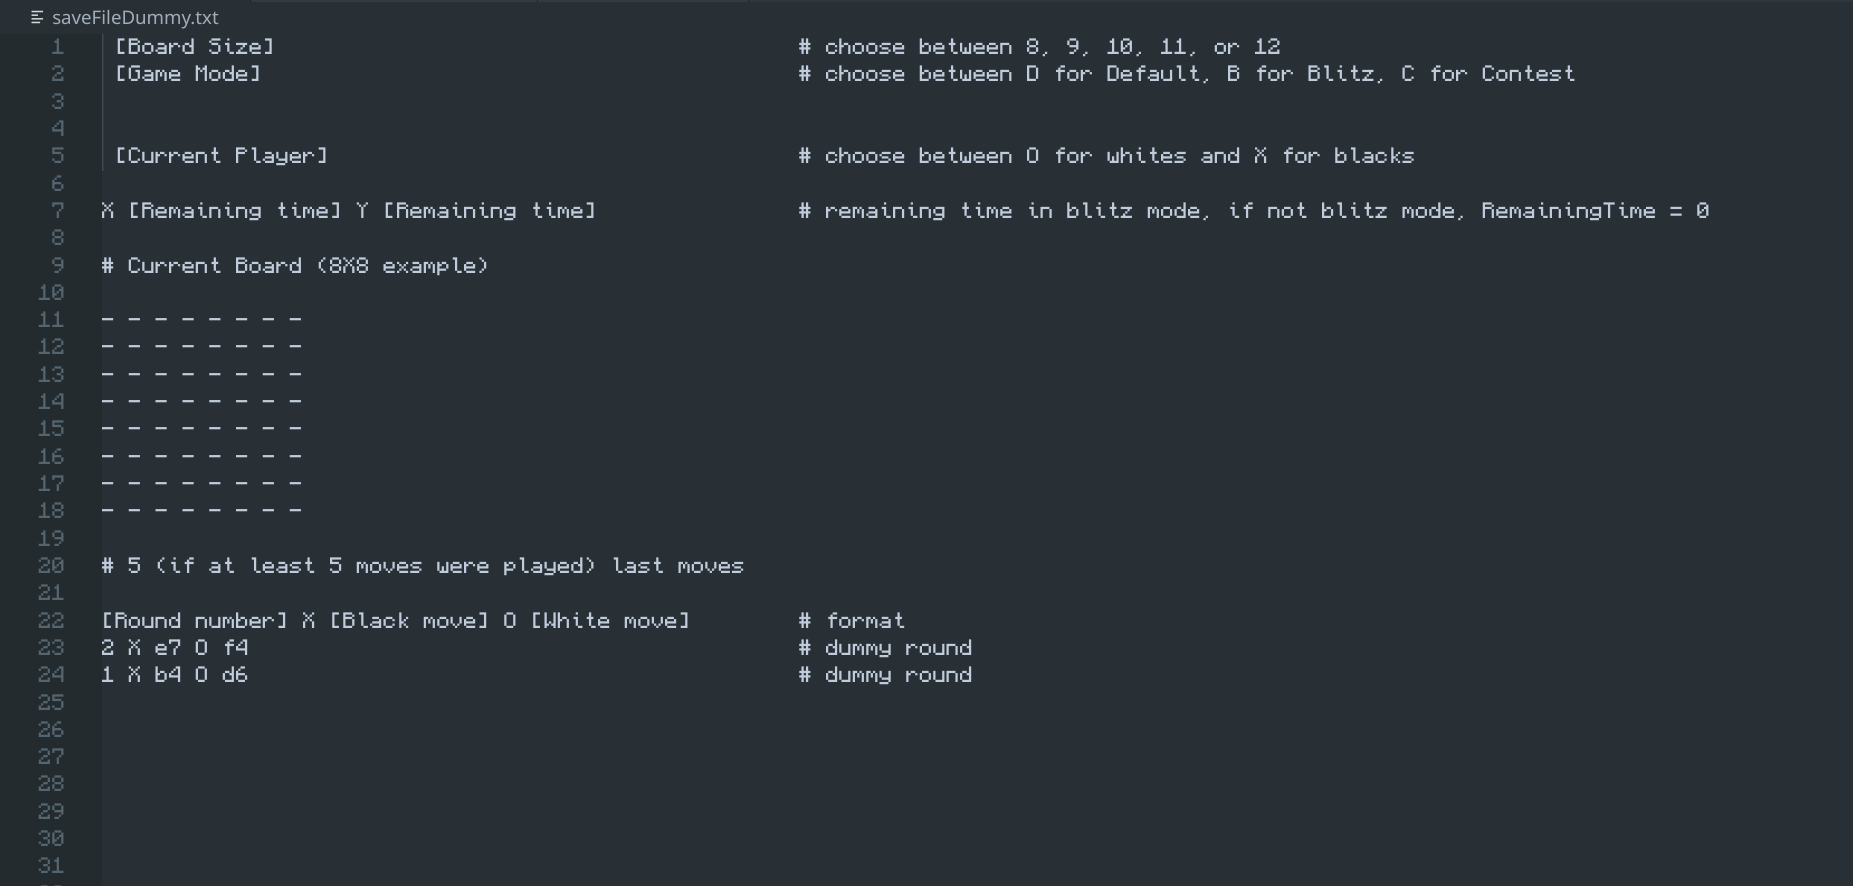
\includegraphics[width=1\linewidth]{images/SaveFileGame.png}
  \caption{Exemple de fichier de sauvegarde d'une partie}
  \label{fig:enter-label}
\end{figure}
\begin{figure}[H]
  \centering
  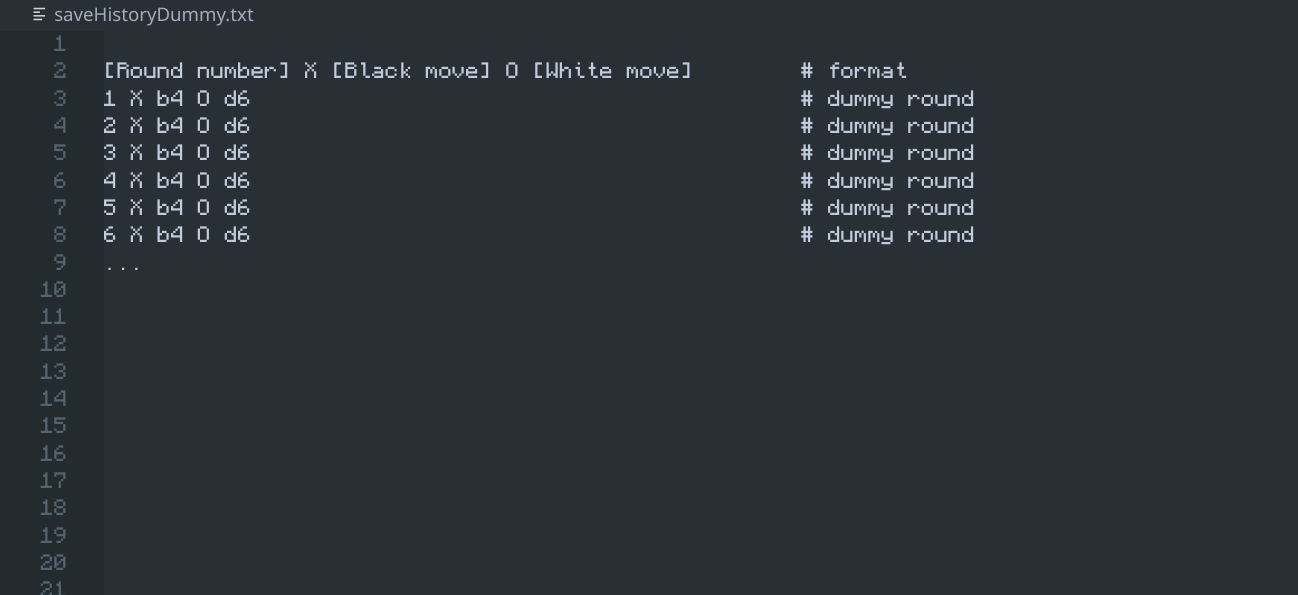
\includegraphics[width=1\linewidth]{images/SaveFileHistory.png}
  \caption{Exemple de ficher Historique des coups}
  \label{fig:enter-label}
\end{figure}

\subsection{Algorithmes utilisés}

Pour la partie Calcul des coups, nous prévoyons d'utiliser l'algorithme Line
Cap Moves, présenté dans \textit{Bitboard Methods for Games, par Cameron
  Browne}:\\ Cet algorithme permet de générer un ensemble de coups possibles dans
chaque direction. C'est-à-dire, donner les emplacements pour lesquels le joueur
courant pourrait capturer des pions adverses dans une direction à la fois.\\
D'abord un ensemble de coups vide est créé, puis on itère sur toutes les
directions: Nord, Nord-Est, Est, Sud-Est, Sud, Sud-West, West, Nord-West.\\
Ensuite, on génère un ensemble de cases 'candidates' par intersection entre les
pions ennemis, et les pions amis shift de 1 sur la direction courante.\\ Tant
que cet ensemble de cases n'est pas vide, on effectue les opérations
suivantes:\\ L'ensemble de coups est actualisé en ajoutant l'intersection entre
l'ensemble vide, et les cases 'candidates' shift de 1 dans la direction. Puis
l'ensemble des cases 'candidates' est réécrit en l'intersection entre lui-même
shift de 1 dans la direction courante, et les pions adverses.\\ Lorsque
l'ensemble de cases 'candidates' est vide, on peut changer de direction et
recommencer. Et quand toutes les directions ont été explorées, l'ensemble de
coups contient tous les coups possibles et légaux.\\

Afin de changer les pions capturés dans la couleur du joueur courant, nous
avons créé un algorithme en se basant sur l'algorithme Line Cap Moves
ci-dessus.\\ En partant de la case sur laquelle le dernier pion a été placé, on
se déplace sur tous les pions ennemis en les retournant pour changer leur
couleur.\\ Tout d'abord, on récupère le dernier pion placé par le joueur
courant, puis on itère dans toutes les directions: Nord, Nord-Est, Est,
Sud-Est, Sud, Sud-West, West, Nord-West.\\ On shift le pion de 1 dans la
direction courante, le pion est donc un pion maintenant Ennemi.\\ Tant que le
pion n'est pas un pion Ami (pion de la couleur du joueur courant), on effectue
les opérations suivantes:\\ Le pion est changé de Ennemi à Ami: on retourne le
pion pour que sa couleur soit celle du joueur courant.\\ Puis on shift le pion
de 1 dans la direction courante.\\ Lorsque le pion sur lequel on s'est déplacé
est un pion Ami, on peut changer de direction et recommencer. Et quand toutes
les directions ont été explorées, tous les pions à capturer ont été changés en
pions du joueur courant.\\

Pour la partie IA, nous allons dans un premier temps utiliser l'algorithme
MiniMax pour choisir le prochain coup joué par le Joueur IA. Minimax est un
algorithme qui parcourt l'arbre représentant les coups possibles, évalue chaque
coup avec l'heuristique de notre choix, et remonte le coup le plus
avantageux.\\ Le 2ème algorithme utilisé est $\alpha\beta$-pruning. Cet
algorithme est très similaire à MiniMax. L'objectif est de parcourir l'arbre
des coups possibles, et d'élaguer certaines branches en déduisant celles qui ne
seront pas utile. Le résultat est le même que celui de Minimax, mais
$\alpha\beta$-pruning est plus efficace car il ne parcourt pas tous les
arbres.\\ L'option "--ai-shallow" sera disponible pour notre
$\alpha\beta$-pruning. L'objectif de cette option est d'explorer notre arbre de
manière peu profonde afin de trier les branches dans l'ordre décroissant
(meilleure branche à gauche, pire branche à droite.). En effectuant ce tri,
$\alpha\beta$-pruning bénéficiera d'un abre trié, ce qui lui permet d'élaguer
des parties plus importantes de l'arbre des coups, aboutissant à un calcul plus
efficace.\\ De plus, plusieurs heuristiques pourront être choisies,
l'algorithme de recherche pourra être raffiné en utilisant
l'$\alpha\beta$-pruning, et une exploration préliminaire.\\

\newpage
\section{Analyse des Besoins}
Ici, nous décrivons les besoins à implémenter pour notre programme.

\subsection{Généralités}

\subsubsection{Besoins non fonctionnels}

\paragraph{F1. Langage de programmation:}
\begin{itemize}
  \item Développer le logiciel en langage Python 3.7+.
\end{itemize}

\paragraph{F2. Style de codage:}
\begin{itemize}
  \item Le code du programme devra suivre le coding style du PEP8.
  \item L'utilisation de pre-commit hooks permettra de s'assurer du respect de ce style
        de codage.
\end{itemize}

\paragraph{F3. Langue par défaut du code}
\begin{itemize}
  \item Le code ainsi que les fichiers seront écrits et commentés en langue anglaise.
\end{itemize}

\paragraph{F4. Système cible:}
Le programme devra fonctionner sur des systèmes d’exploitation GNU/Linux.
\begin{itemize}
  \item Développer le logiciel sous une distribution Linux.
  \item Tester sous une distribution Linux Debian et une distribution Ubuntu.
  \item Sur un système Debian récent, il sera nécessaire de passer par un environnement
        virtuel car l'intégration de python rend compliqué voir impossible
        l'installation de modules python sur l'environnement par défaut.
\end{itemize}

\paragraph{F5. Documentation:}
\begin{itemize}
  \item Un manuel utilisateur sera à disposition de l'utilisateur, ainsi qu'une
        description des options d'aide.
\end{itemize}

\paragraph{F6. Tests:}
\begin{itemize}
  \item Les tests couvriront au moins 80\% du code.
  \item Tous les tests seront automatisés. Le coverage sera également intégré à la
        pipeline CI gitlab.
\end{itemize}

\paragraph{F7. Bugs:}
\begin{itemize}
  \item Dans la mesure du possible, nous ferons en sorte de n'avoir aucun bug qui
        ferait crash notre implémentation.
\end{itemize}

\paragraph{F8. Performances:}
\begin{itemize}
  \item Les performances seront mesurées en temps, en utilisant le module python
        timeit.
\end{itemize}

\subsection{Bibliothèque et outils}

\subsubsection{Besoins fonctionnels}

\paragraph{F11. Gestion des options:}
\begin{itemize}
  \item Les options en lignes de commandes seront gérées par le module argparse qui,
        une fois proprement configuré par le code, construit un objet contenant les
        arguments.
  \item Les arguments passés au programme prendront systématiquement la priorité sur
        les paramètres définit dans le fichier de configuration othello qui lui même
        aura la priorité sur les paramètres par défaut.
\end{itemize}

\subsubsection{Besoins non fonctionnels}

\paragraph{F9. Build-system:}
\begin{itemize}
  \item Le build-system sera basé sur pyproject.toml et setuptools.
\end{itemize}

\paragraph{F10. Framework de tests:}
\begin{itemize}
  \item Nous utiliserons le framework de test Pytest ainsi que Coverage.
\end{itemize}

\paragraph{F12. Bibliothèque graphique:}
\begin{itemize}
  \item La bibliothèque graphique utilisée sera basée sur PyGObjet.
\end{itemize}

\subsection{Options en ligne de commande}

\subsubsection{Besoins fonctionnels}

\paragraph{F15. Usage général:}
\begin{itemize}
  \item Pour l'interface en ligne de commande, nous utiliserons les outils offerts par
        l'API de python (input, print...).
  \item Nous utiliserons la bibliothèque graphique PyGObject, un portage python de la
        librairie GLib Object System, une librairie portée par le projet GNOME à la
        base de librairies graphiques telles que GTK.
        \paragraph{Sous Besoins:}
  \item Nous aurons besoins d'utiliser différentes classes offertes par la librairie
        afin de gérer l'affichage de la fenêtre principale afin d'afficher la fenêtre,
        le board, l'historique ainsi que quelques boutons et pop-up de confirmation.
\end{itemize}

\paragraph{F16. Aide en ligne de commande:} Les options '-h' et '--help' affichent l'aide puis quittent.
\begin{itemize}
  \item Tester que les deux commandes affichent bien l'aide.
  \item Tester que pour les deux terminent bien avec EXIT\_SUCCESS.
\end{itemize}

\paragraph{F17. Version:} Les options '-V' et '--version' affichent la version puis quittent.
\begin{itemize}
  \item Tester que les deux commandes affichent bien la version.
  \item Tester que les deux commandes terminent bien avec EXIT\_SUCCESS.
\end{itemize}

\paragraph{F19. Debug:} Les options '-d' et '--debug' affichent des informations de debogage pendant
l'exécution.
\begin{itemize}
  \item Affichage des informations supplémentaires au cours de la partie.
\end{itemize}

\paragraph{F21. Blitz:} Les options '-b' et '-blitz' permettent de jouer en mode blitz.
\begin{itemize}
  \item Un temps limite sera imposé au joueur pour la partie. Le temps écoulé donnera
        la victoire au joueur adverse.
\end{itemize}

\paragraph{F22. Durée du Blitz:} Les options '-t TIME' et '-time TIME' Permettent de spécifier la durée fixée
pour chaque coup en mode Blitz.
\begin{itemize}
  \item Si l'option est utilisée sans l'option Mode Blitz, elle sera ignorée.
  \item Par défaut, la durée limite sera de 30 minutes.
        \paragraph{Sous Besoins}
  \item Le mode Blitz devra être implémenté.
\end{itemize}

\paragraph{F23. Contest:} Les options '-c FILENAME' et '-contest FILENAME' Permettent de charger une
partie.
\begin{itemize}
  \item Un affichage du joueur et du coup précédent joué.
\end{itemize}

\paragraph{F24. Mode IA:}
\begin{itemize}
  \item Possibilité de lancer une partie contre une intelligence artificielle. On
        pourra éventuellement préciser la ou les couleurs contrôlées par IA. Par défaut
        elle contrôlera le joueur aux pions noirs.
\end{itemize}

\subsubsection{Besoins non fonctionnels}

\paragraph{F14. Nom du programme:}
\begin{itemize}
  \item l'exec principal s'appellera 'othello'.
  \item et lancera tout le programme.
        \paragraph{Sous Besoins:}
  \item Afin de lancer le programme, nous aurons besoin d'un environnement virtuel.
\end{itemize}

\subsection{Interface utilisateur}

\subsubsection{Besoins fonctionnels}

\paragraph{F25. Interface en ligne de commande (CLI):}
\begin{itemize}
  \item L'affichage se fera toujours à minima dans le terminal.
  \item Au lancement, les informations respectives de la partie - issues soit des
        fichiers de configuration soit des paramètres passés à l'exécutable - seront
        rappelées.
  \item Pour chaque tour, nous afficherons de haut en bas:
        \begin{itemize}
          \item L'en tête d'un tour rappelant le type de partie (Joueur vs Joueur, IA vs
                Joueur, IA vs IA) ainsi que le mode de jeu (normal, blitz ou contest).
          \item Si la partie est en mode blitz, le temps restant pour chaque joueur (F27)
          \item Le plateau de jeu en ASCII (F27)
          \item Les 5 derniers coups joués
          \item Un invite pour que l'utilisateur puisse effectuer des actions
          \item Pour tester ce besoin, nous allons simplement comparer l'affichage sur la
                sortie standard d'états de jeu prédéfinis en utilisant le module "capsys".
        \end{itemize}
\end{itemize}

\paragraph{F25 Bis. Invite de commande}
\begin{itemize}
  \item Pour effectuer une action en mode CLI, l'utilisateur sera invité à rentrer une
        commande parmi :
        \begin{itemize}
          \item "?", qui lui rappelera les commandes possibles
          \item "r" qui lui rappelera les règles du jeu
          \item Un coup sous la forme "[a-h][1-8]"
          \item "s" pour sauvearder et quitter la partie (une confirmation sera demandée sous la forme [Y/N])
          \item "sh" pour sauvegarder l'historique de la partie
          \item "ff" pour abandonner la partie (une confirmation sera demandée sous la forme [Y/N])
          \item "restart" pour relancer la partie dans les même conditions
          \item Le parser prendra une string et renverra une instance de l'enum "Command"
                paramétrée qui sera ensuite interprétée par le contrôlleur.
          \item Pour tester ce besoin, nous allons passer des chaînes de caractère à la
                fonction parse et regarder quelle en est la Command résultante.
        \end{itemize}
\end{itemize}

\paragraph{F26. Interface graphique:} Les options '-g' et '--gui' permettront d'ouvrir une interface graphique.
\begin{itemize}
  \item L'interface graphique affichera le plateau de jeu.
  \item L'interface graphique affichera un historique des coups joués.
  \item L'interface graphique affichera le joueur dont c'est le tour de jouer.
  \item Si l'option est passée en argument, c'est le main qui se chargera d'instancier
        une interface graphique en plus de l'interface CLI
  \item Pour tester ce besoin, nous vérifierons que l'objet de configuration assigne la
        bonne valeur au paramètre représentant l'affichage de la GUI.
\end{itemize}

\paragraph{F29. Représentation de l'historique}
\begin{itemize}
  \item L'historique affichera les 5 derniers coups joués sous le format:\\ "\{numéro
        de tour\} X \{coup\} O \{coup\}"
  \item L'historique sera géré par une liste python dans le contrôlleur du jeu.
  \item Pour tester ce besoin, nous préparerons des parties dans un état prédéfini et
        compareront l'état de la liste du contrôlleur avec la valeur que nous en
        attendons.
\end{itemize}

\paragraph{F30. Abandon:} Le joueur peut abandonner une partie en cours de jeu.
\begin{itemize}
  \item Dans le terminal de commande, le joueur pourra abandonner une partie en entrant
        'ff'.
  \item Une question sera posée au joueur pour qu'il vérifie l'action avec [Y/N].
  \item L'abandon donne la victoire au joueur adverse, puis quitte la partie.
  \item Cela se traduira en l'arrêt de la boucle de jeu dans le main
  \item Pour tester ce besoin, nous appelerons la fonction d'abandon et nous
        regarderons si l'état du jeu a bien changé. La boucle se basant sur l'état du
        jeu pour savoir si une partie est finie où non cela sera suffisant.
\end{itemize}

\paragraph{F31. Affichage des messages}
\begin{itemize}
  \item En mode CLI, les messages seront affichés dans la console. Ils seront forcément
        en dessous de l'organisation décrite dans le paragraphe F25.
  \item En mode GUI, les message s'afficheront dans un label en bas de l'écran.
  \item Les messages seront des messages informatifs pour l'utilisateur, lui signifiant
        une erreur d'utilisation et éventuellement des messages de debug si l'option
        est activée.
  \item Pour tester l'affichage des messages, nous testerons à différents niveaux
        d'affichage (normal / debug) si l'envoi de messages résulte bel et bien en
        l'ajout de messages à la liste des messages gérés par le jeu.
\end{itemize}

\paragraph{F32. Quitter et Sauvegarder une partie:} Le joueur peut quitter une partie en cours de jeu.
\begin{itemize}
  \item Dans le terminal de commande, le joueur pourra sauvegarder puis quitter une
        partie en entrant 'Q' puis en confirmant ou non avec [Y/N].
  \item Une sauvegarde du jeu dans son dernier état sera faite, puis la partie sera
        quittée.
  \item Le joueur sera notifié de l'emplacement de fichier dans lequel la partie a été
        sauvegardée.
  \item Pour tester ce besoin, nous placerons le jeu dans un état donné, lanceront
        manuellement (en appelant les fonctions de save) une sauvegarde puis chargerons
        les fichiers résultants et vérifierons leur conformité en les comparant à la
        valeur attendue.
\end{itemize}

\paragraph{F33. Sauvegarde de l'historique}
\begin{itemize}
  \item Dans le terminal de commande, le joueur pourra l'historique de la partie en
        tapant "sh".
  \item Dans l'interface graphique, le joueur aura un bouton pour sauvegarder
        l'historique de la partie.
  \item Pour tester ce besoin, nous jouerons un certain nombre de coups dans le test de
        manière programmatique pour ensuite exporter une sauvegarde et vérifier qu'elle
        est conforme à nos attentes.
\end{itemize}

\paragraph{F35. Recommencer une partie}
\begin{itemize}
  \item Dans le terminal, le joueur pourra recommencer une partie en tapant "restart".
        Il lui sera demandé une confirmation.
  \item Dans l'interface graphique, le joueur aura un bouton restart. Il lui sera
        demandé une confirmation.
  \item Pour tester ce besoins, nous partirons d'un état donné, lancerons un restart et
        vérifierons que l'état du jeu a bien été réinitialisé.
\end{itemize}

\paragraph{F36. Fin de partie:} Le programme doit détecter une fin de partie.
\begin{itemize}
  \item La partie se termine si aucun pion ne peut être posé sur l'othellier.
  \item La partie se termine si aucun des deux joueurs ne peut captuere de pions
        adverses en posant un pion.
  \item Le gagnant est le joueur ayant le plus de pions sur l'othellier. Dans le cas où
        les deux jouaurs auraient le même nombre de points, la partie se termine en une
        égalité.
  \item Pour tester ce besoin, nous préparerons des parties à un coup de la fin de
        partie, jouerons le coup et vérifierons que la partie est bien dans un état
        terminé.
\end{itemize}

\subsubsection{Besoins non fonctionnels}

\paragraph{F28. Notation des coups:}
\begin{itemize}
  \item Un coup sera noté sous la forme: [a-h][1-8].
  \item Si le coup n'est pas valide, on le notifie au joueur et demande un autre coup.
  \item S'il n'y a pas de coups possibles pour le joueur courant, on le notifie au
        joueur, et son tour sera passé.
\end{itemize}

\subsection{Formats d'entrée - sortie}

\subsubsection{Besoins non fonctionnels}

\paragraph{F38. Format de fichier simplifié:} Les fichiers de partie seront en format ASCII simplifié.
\begin{itemize}
  \item Les fichiers contiendront la sauvegarde d'une partie de jeu.
  \item Les fichiers pourront être chargés afin de reprendre la partie depuis l'état
        décrit dans le fichier.
  \item Le fichier de sauvegarde contiendra le mode de jeu, le temps de jeu restant à
        chaque joueur, le joueur courant, l'état du plateau, l'historique des cinq (ou
        moins si moins de cinq coups ont été joués avant la sauvegarde) derniers coups
        joués.
  \item Vérifier que
\end{itemize}

\paragraph{F39. Format de l'historique}
\begin{itemize}
  \item La sauvegarde se fera au travers de fichiers .othelloc.
  \item Il ne contiendra que les coups joués et d'éventuels commentaires et ne
        permettra pas de reprendre une partie.
  \item Vérifier que le fichier d'historique est vide au début d'une partie.
  \item Vérifier que l'historique des coups est bien écrit dans le fichier d'historique
        pour quelques coups.
  \item Vérifier que les coups sont écrits dans le fichier d'historique en respectant
        le format spécifié.
\end{itemize}

\paragraph{F40. Fichier de configuration:} Un fichier .othellorc contiendra les options utilisées dans une partie.
\begin{itemize}
  \item Les options indiquées seront utilisées par défaut dans le jeu.
  \item Si des options sont passées en ligne de commande, elles remplaceront les
        options par défaut du fichier de configuration.
  \item Le fichier sera au format INI.
  \item Le fichier définira les options par défaut pour le lancement d'une partie
        simple: pas d'ia, pas de mode blitz ni contest, plateau de taille
        réglementaire.
  \item Vérifier que le fichier de configuration par défaut contient toutes les
        options, et qu'elles sont bien initialisées avec leurs valeurs par défaut.
  \item Vérifier que lorsque l'on change une option, le fichier de configuration soit
        modifié.
\end{itemize}

\subsection{Structure interne}

\subsubsection{Besoins fonctionnels}

\paragraph{F41. Plateau de jeu:}
\begin{itemize}
  \item Le plateau de jeu sera représenté en utilisant des bitboard.
  \item Nous aurons deux bitboard représentant les pions des joueurs.
  \item Nous aurons également un masque par côté afin d'éviter les effets de bord liés
        aux décalages.
  \item Nécessaire d'avoir le module BitBoard implémenté.
  \item Vérifier avec plusieurs plateaux différents (différentes tailles) que le
        plateau de jeu est correctement représenté par les bitboards.
  \item Vérifier (avec différentes tailles de plateaux) que le plateau de jeu au début
        d'une partie est correctement initialisé avec les 4 premiers pions placés
        correctement.
  \item Vérifier après un coup joué que le plateau de jeu a bien ajouté un pion et
        capturé les pions ennemis.
\end{itemize}

\paragraph{F42. Module Bitboard:}
\begin{itemize}
  \item Le module Bitboard sera utilisé afin de représenter le plateau de jeu.
  \item Deux masques seront utilisés pour représenter les pions de chaque couleurs.
  \item Deux masques seront utilisés pour représenter les colonnes de droite et gauche,
        afin de gérer les cas de wrapping.
  \item Vérifier que les opérations renvoient bien le résultat désiré.
  \item Vérifier les effets de bords lors des shifts sur la droite ou la gauche.
\end{itemize}

\paragraph{F43. Etat du jeu}
\begin{itemize}
  \item L'état courant du jeu se chargera de garder:
        \begin{itemize}
          \item Le joueur courant.
          \item Le temps restant à jouer si le mode de jeu est blitz.
          \item L'état du plateau qui sera géré par une implémentation d'un plateau d'othello
                utilisant des bitboard.
          \item L'historique des coups joués.
          \item Vérifier l'état du jeu avec un jeu qui vient d'être lancé.
          \item Vérifier que l'état du jeu est actualisé après avoir joué un coup: board
                actualisé, historique des coups actualisé, changement de joueur courant.
          \item Vérifier que le temps est bien décompté en mode blitz.
          \item Vérifier avec plus de 6 coups joués que l'historique garde bien les 5 derniers
                coups.
        \end{itemize}
\end{itemize}

\subsection{Interface graphique}

\subsubsection{Besoins fonctionnels}

\paragraph{F44. Fonctions de base:}
\begin{itemize}
  \item L'interface graphique devra permettre au joueur d'utiliser toutes les
        fonctionnalités présentes dans l'interface en ligne de commande.
  \item Les coups devront être joués en plaçant un pion sur le plateau affiché.
  \item Un historique des derniers coups sera présent sur l'ui.
        \paragraph{Sous Besoins}
  \item Nécessite une interface graphique (F26.).
  \item Afficher un plateau sur l'UI.
  \item Afficher les pions sur le plateau.
  \item Afficher le joueur courant.
  \item Afficher les cinq (ou moins) derniers coups joués.
  \item Tester que l'interface graphique affiche correctement le plateau prédéfinit.
  \item Tester que l'interface affiche bien le joueur courant, et change de joueur
        courant après un coup.
\end{itemize}

\paragraph{F49. Affichage des coups joués}
\begin{itemize}
  \item Les 5 derniers coups seront affichés en dessous du plateau à la fois pour
        l'affichage CLI et GUI.
  \item Tester que l'historique affiche les coups correspondants dans le bon ordre.
\end{itemize}

\subsection{Joueur artificiel}

\subsubsection{Besoins fonctionnels}

\paragraph{F51/F57. Heuristique d'évaluation de position + Choix des heuristiques}
\begin{itemize}
  \item Le jeu aura une heuristique qui pourra prendre plus ou moins de paramètres en
        compte afin d'avoir un choix du niveau de difficulté de l'heuristique.
  \item Tester que la fonction heuristique sélectionnée renvoit le score d'évaluation
        anticipé pour un board donné.
\end{itemize}

\paragraph{F52. Algorithme de recherche MiniMax:}
\begin{itemize}
  \item Option utilisée par défaut par l'IA lorsque le jeu est lancé en mode IA.
  \item Une profondeur maximale pour l'arbre de recherche utilisé sera définie par
        défaut.
        \paragraph{Sous Besoins}
  \item Nécessite au moins une fonction d'heuristique d'évaluation d'un plateau.
  \item Tester que la fonction Minimax renvoit le meilleur coup théorique pour une
        profondeur et un board donné.
\end{itemize}

\paragraph{F53. $\alpha\beta$-pruning}
\begin{itemize}
  \item En plus de l'algorithme Minimax, on pourra utiliser de l'$\alpha\beta$-pruning
        qui pourra remplacer minimax pour le joueur artificiel.
  \item Idem que la fonction Minimax : Tester la fonction $\alpha\beta$ et vérifier si
        elle renvoit le meilleur coup théorique pour un board et profondeur donnée.
\end{itemize}

\paragraph{F54. Exploration peu profonde préliminaire:} L'option '--ia-shallow' active une exploration préliminaire de l'arbre de
recherche, et ordonne les coups selon leur priorité
\begin{itemize}
  \item Effectue un tri des plateaux évalués.
  \item L'arbre de recherche trié sera utilisé pour déterminer le meilleur coup plus
        rapidement.
  \item Vérifier que l'$\alpha\beta$-pruning trouve le meilleur coup théorique en un
        meilleur temps avec l'option '--ai-shallow' que la même fonction sans l'option
        active.
\end{itemize}

\paragraph{F56. Profondeur de recherche:} L'option '--ai-depth DEPTH' spécifiera une profondeur maximale.
\begin{itemize}
  \item La profondeur spécifiée remplacera la profondeur par défaut.
  \item Si la profondeur spécifiée est trop large, la profondeur utilisée sera la
        valeur de la borne haute calculée.
        \paragraph{Sous Besoins}
  \item Borner la profondeur par une valeur large, mais pas assez large pour prendre
        trop de temps.
  \item Nécessite de calculer/tester sur des grandes valeurs les performances de l'ia.
  \item Tester que la fonction sélectionnée (Minimax ou $\alpha\beta$-pruning) trouve
        le coup théorique correspondant à la profondeur demandée.
\end{itemize}

\paragraph{F58. Calcul des libertés:}
\begin{itemize}
  \item Utilisation de l'opération de dilatation sur les bitboards.
  \item Calcul des cases vides en contact avec un pion du joueur courant.
  \item Tester que la fonction calcule le bon degré de liberté d'une pierre donnée.
\end{itemize}

\paragraph{F60. Temps de réflexion borné:} l'option '--ai-time TIME spécifie le temps de réflexion de l'algorithme de
recherche.
\begin{itemize}
  \item Spécifie une borne de temps à l'algorithme de recherche de l'IA. Cette valeur
        remplace la valeur par défaut.
  \item La valeur par défaut du temps de réflexion est de 05 secondes.
  \item Si le temps est écoulé avant que l'algorithme ne termine, le plateau 'le mieux
        évalué pour le moment' doit être renvoyé comme meilleur plateau.
        \paragraph{Sous Besoins}
  \item Nécessaire de garder le plateau 'le mieux évalué pour le moment' au cours de
        l'algorithme de recherche.
  \item Nécessaire de tester le temps de réflexion restant à l'IA au cours de
        l'algorithme de recherche.
  \item Tester que la fonction sélectionnée (Minimax ou $\alpha\beta$-pruning) trouve
        le meilleur coup en un temps déterminé.
\end{itemize}

\newpage
\section{Architecture}
\begin{figure}[H]
  \centering
  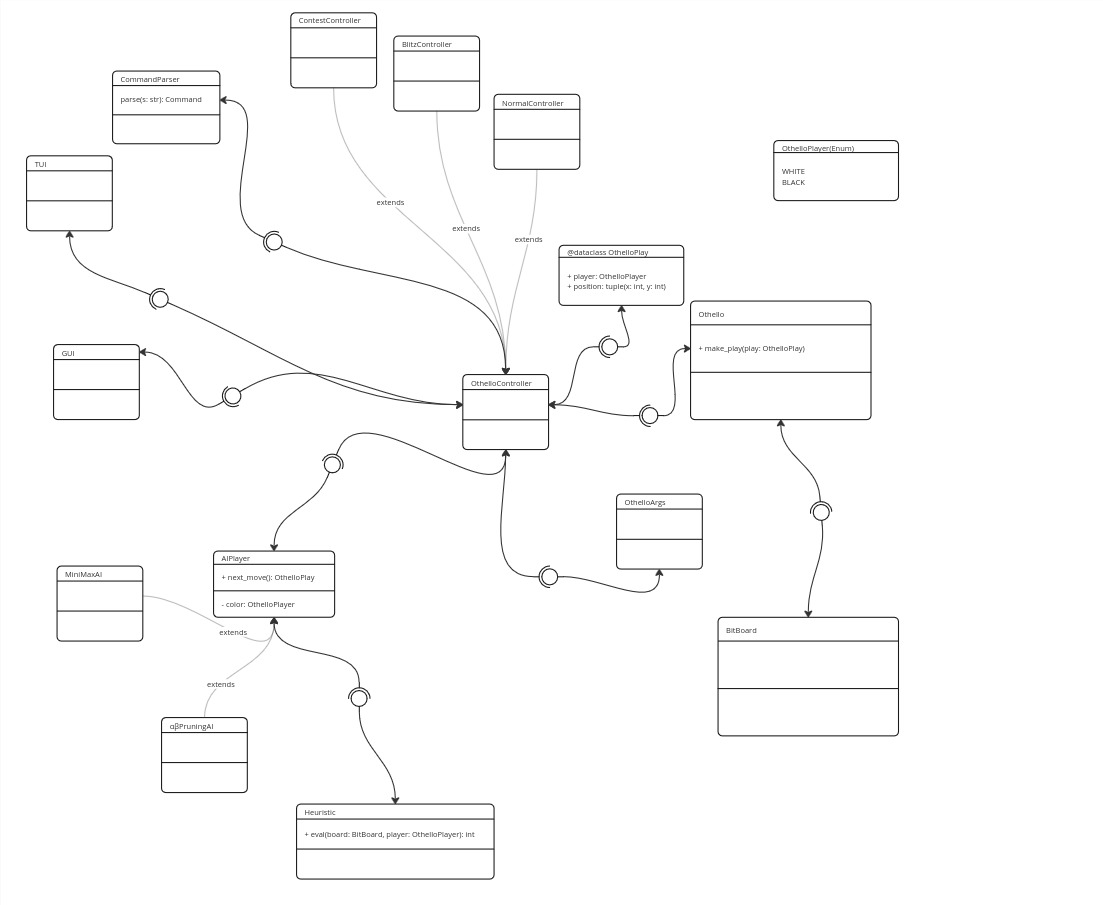
\includegraphics[width=1\linewidth]{images/diag_classe.jpg}
  \caption{Diagramme de classe}
  \label{fig:enter-label}
\end{figure}

Trois modules principaux ressortent de cette architecture.\\ Un module
"othello\_logic" qui regroupe la logique de jeu d'Othello, les BitBoards
utilisés, ainsi que quelques éléments tels qu'une Enum représentant la couleur
du joueur en cours ou encore la représentation d'un coup.\\ Un module
"othello\_interfaces" qui interface la logique de jeu et le joueur, à la fois à
travers trois contrôlleurs - un par mode de jeu - et également les vues de CLI
(TUI) et GUI qui intéragissent directement avec le contrôlleur utilisé selon la
configuration de la partie, et un module "ai" qui contient à la fois la logique
des différentes IA implémentées ainsi que l'heuristique.\pagebreak

Un quatrième module, ne figurant pas sur le diagramme mais étant implicit à la
majorité des programmes, sera le module définissant notamment le main. Il
récupèrera le fichier de configuration si il existe, parsera les éventuels
arguments avec argparse et instanciera le bon contrôlleur et les bonnes vues.
Il contiendra également la boucle de jeu.

\section{Mockup de l'interface graphique}
\begin{figure}[H]
  \centering
  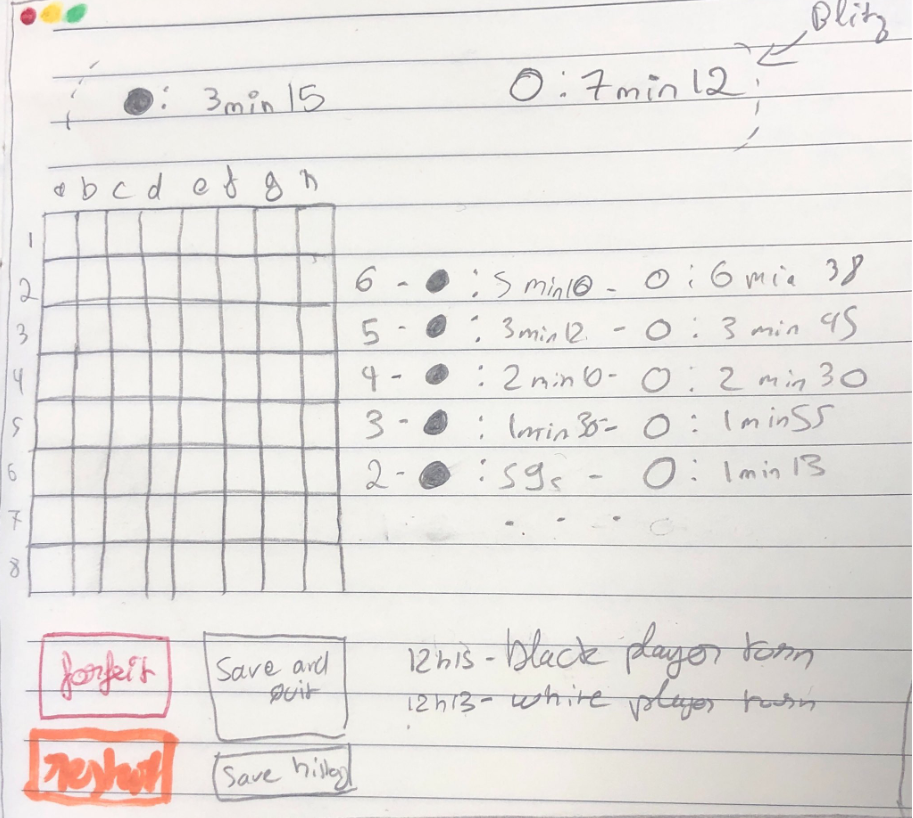
\includegraphics[width=1\linewidth]{images/mockup.png}
  \caption{Mockup de l'interface graphique}
  \label{fig:mockup-interface-graphique}
\end{figure}

\newpage
\section{Outils de gestion de projet}

Du côté de la gestion de projet, nous utilisons GitLab comme dépôt de code,
afin de pouvoir travailler à plusieurs sur différentes ou sur les mêmes
fonctionnalités de manière efficace. De plus, nous allons utiliser une pipeline
de CI gitlab nous permettant d'automatiser le lancement des tests et la
vérification du coverage.\\ Notre utilisons un diagramme de Gantt pour suivre
notre agenda prévisionnel.\\ Et nous utilisons un tableau sur Miro pour
brainstorm sur les besoins de notre projet.\\

\section{Planification}
%\subsection{Échéancier}
Voici notre agenda prévisionnel semaine par semaine. Les besoins à livrer sont
listés, avec leurs dépendances et le temps prévu pour les implémenter. Notre
Gantt a code couleur qui est le suivant:
\begin{itemize}
  \item Orange, Lucas Zammit
  \item Vert, Rémy Heuret
  \item Rose, Lucas Marques
  \item Violet, Matis Duval
  \item Bleu, Gabriel Tardiou
\end{itemize}

\\

\begin{figure}[H]
  \centering
  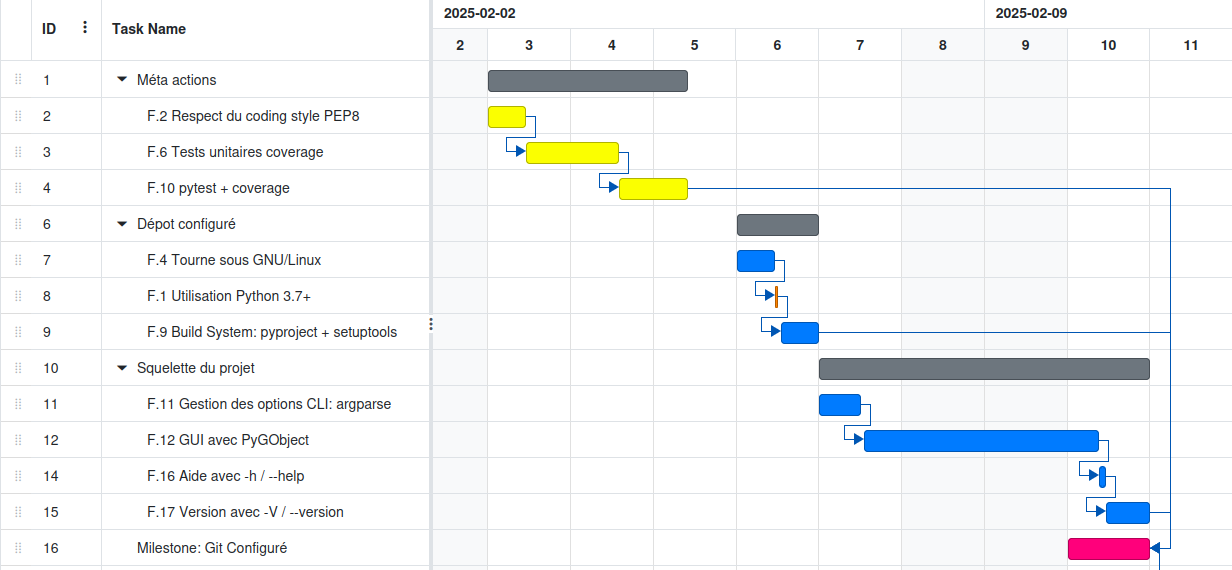
\includegraphics[width=18cm]{images/Semaine1.png}
  \caption{Agenda prévisionnel Première semaine}
\end{figure}

\begin{figure}[H]
  \centering
  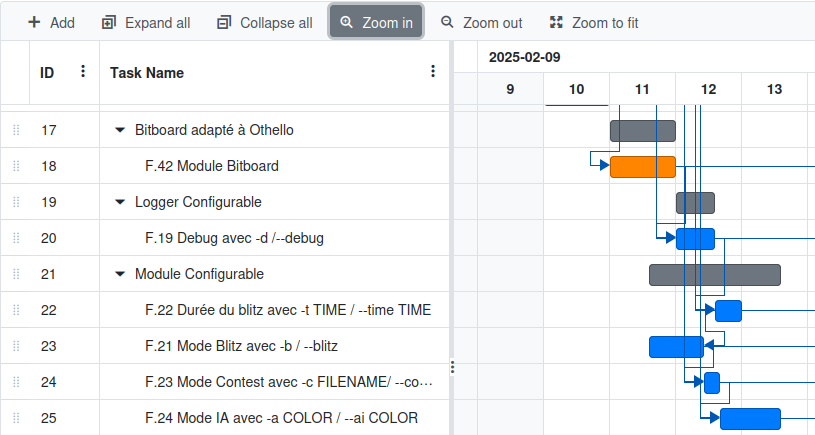
\includegraphics[width=18cm]{images/Semaine2.png}
  \caption{Agenda prévisionnel Seconde semaine}
\end{figure}

\begin{figure}[H]
  \centering
  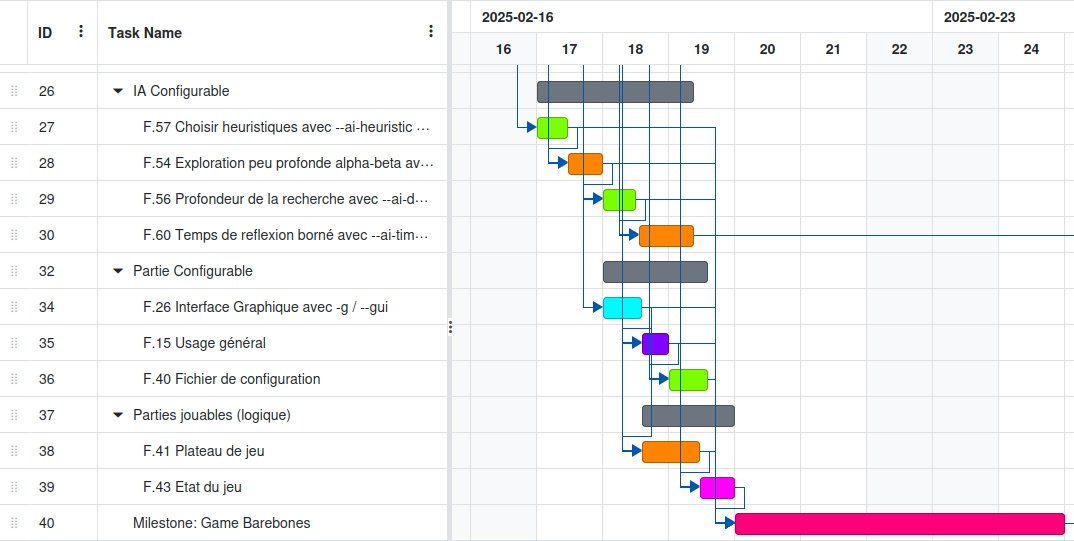
\includegraphics[width=18cm]{images/Semaine3.png}
  \caption{Agenda prévisionnel Troisième semaine}
\end{figure}

\begin{figure}[H]
  \centering
  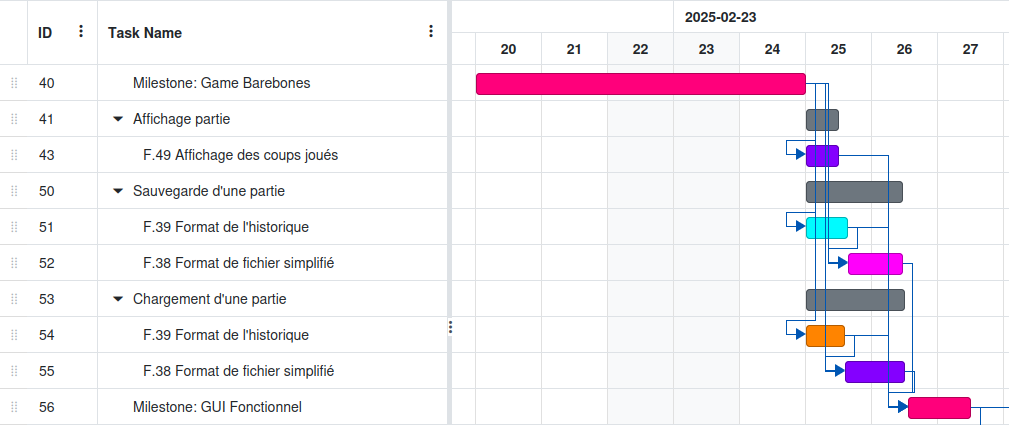
\includegraphics[width=18cm]{images/Semaine4.png}
  \caption{Agenda prévisionnel Quatrième semaine}
\end{figure}

\begin{figure}[H]
  \centering
  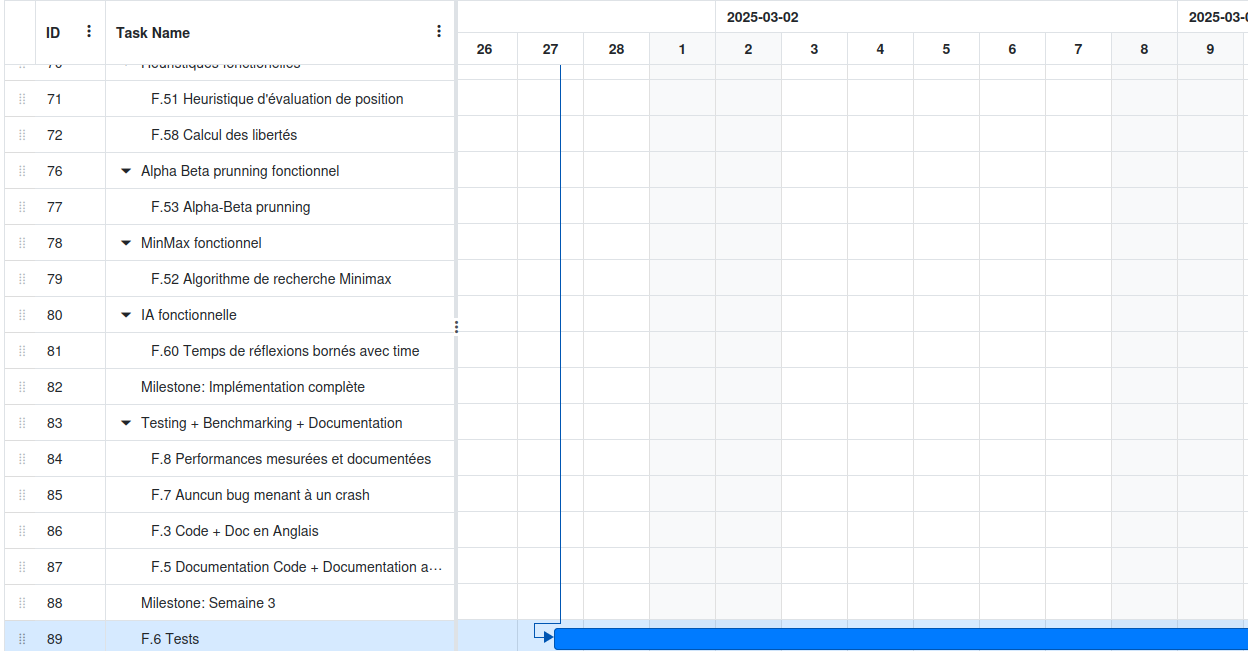
\includegraphics[width=18cm]{images/Semaine5.png}
  \caption{Agenda prévisionnel Cinquième semaine}
\end{figure}

\begin{figure}[H]
  \centering
  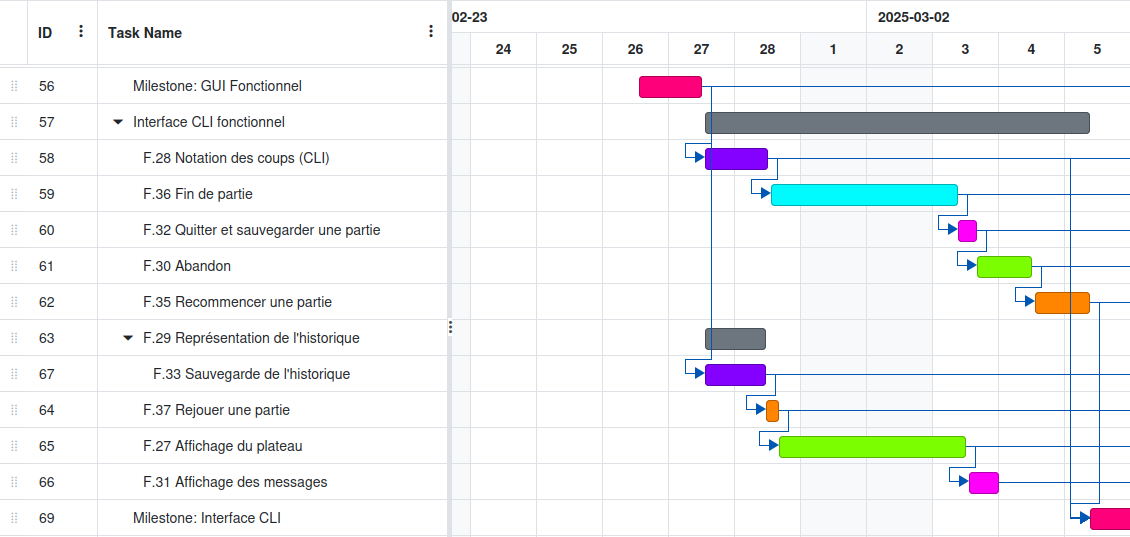
\includegraphics[width=18cm]{images/Semaine6.png}
  \caption{Agenda prévisionnel Sixième semaine}
\end{figure}

\begin{figure}[H]
  \centering
  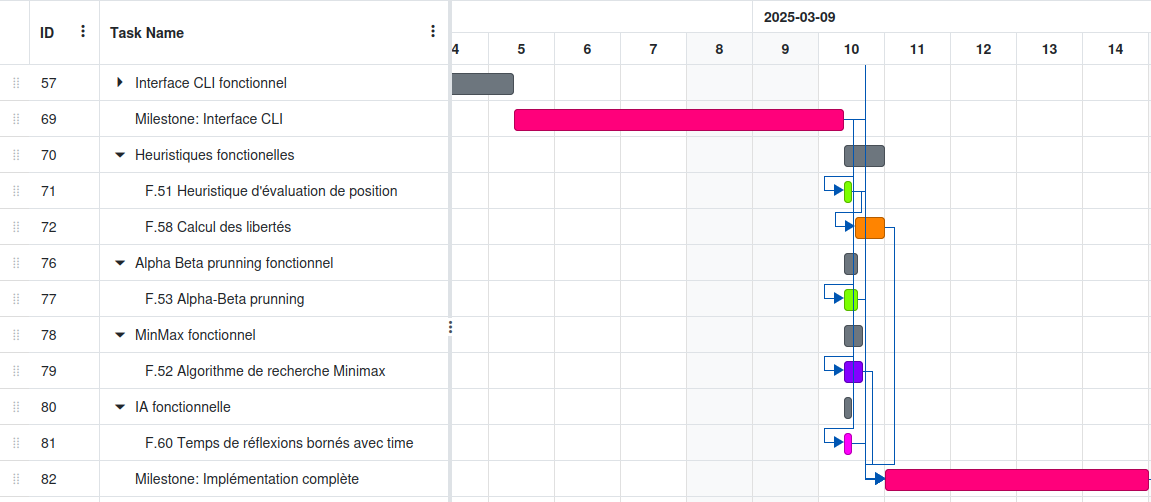
\includegraphics[width=18cm]{images/Semaine7.png}
  \caption{Agenda prévisionnel Septième semaine}
\end{figure}

\begin{figure}[H]
  \centering
  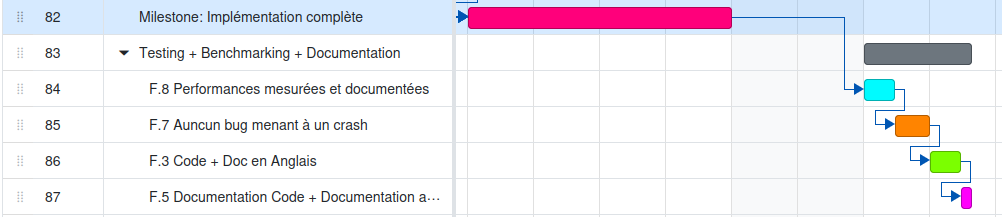
\includegraphics[width=18cm]{images/Semaine8.png}
  \caption{Agenda prévisionnel Huitième semaine}
\end{figure}

\newpage
\section*{Annexes}
%Inclure des annexes si nécessaire : diagrammes supplémentaires, documentation technique, etc.

\subsection*{Bibliographie}
La bibliographie est incluse ci-dessous :

% Articles scientifiques
\begin{thebibliography}{10}

  \bibitem{reversi}
  Wikipedia, Reversi
  \url{https://en.wikipedia.org/wiki/Reversi}

  \bibitem{takizawa2023}
  Hiroki Takizawa,
  \emph{Othello is Solved},
  2023.

  \bibitem{browne2014}
  Cameron Browne,
  \emph{Bitboard Methods for Games},
  2014.

  \bibitem{sannidhanam}
  Vaishnavi Sannidhanam and Muthukaruppan Annamalai,
  \emph{An Analysis of Heuristics in Othello}.

  % Ressources en ligne
  \bibitem{chess-programming}
  Chess Programming Wiki,
  \emph{Bitboards},
  \url{https://www.chessprogramming.org/Bitboards},
  \bibitem{rgbcube-gitignore}
  RGB Cube, .gitignore is inherently sisyphean
  \url{https://rgbcu.be/blog/gitignore/},

  \bibitem{gitlab-ci}
  GitLab Documentation,
  \emph{GitLab CI/CD},
  \url{https://docs.gitlab.com/ee/ci/},

  \bibitem{pygobject}
  PyGObject Documentation,
  \url{https://pygobject.gnome.org/},

\end{thebibliography}
\end{document}
